% Figure 1: system architecture. Compile on its own:  pdflatex architecture.tex
% Drawn at final size (7 in wide) so the type matches the paper's 7pt figure text.
\documentclass[border=1pt]{standalone}
\usepackage[T1]{fontenc}
\usepackage{libertine}
\usepackage{tikz}
\usetikzlibrary{arrows.meta,calc,positioning}

\definecolor{ink}{HTML}{1F2328}
\definecolor{muted}{HTML}{5B6470}
\definecolor{line}{HTML}{8B94A1}
\definecolor{lane}{HTML}{F5F6F8}
\definecolor{lanerule}{HTML}{D3D8DF}
\definecolor{store}{HTML}{E9ECF1}
\definecolor{accent}{HTML}{1F4E79}
\definecolor{accentfill}{HTML}{E3ECF6}
\definecolor{warm}{HTML}{9A4A12}
\definecolor{warmfill}{HTML}{FBEEDF}

\newcommand{\fs}{\fontsize{6.8}{7.9}\selectfont}
\newcommand{\fsmall}{\fontsize{6}{7}\selectfont}
\newcommand{\ftitle}{\fontsize{5.8}{7}\selectfont\bfseries}
\newcommand{\wnum}[1]{\textcolor{accent}{\textbf{#1}}}

\begin{document}
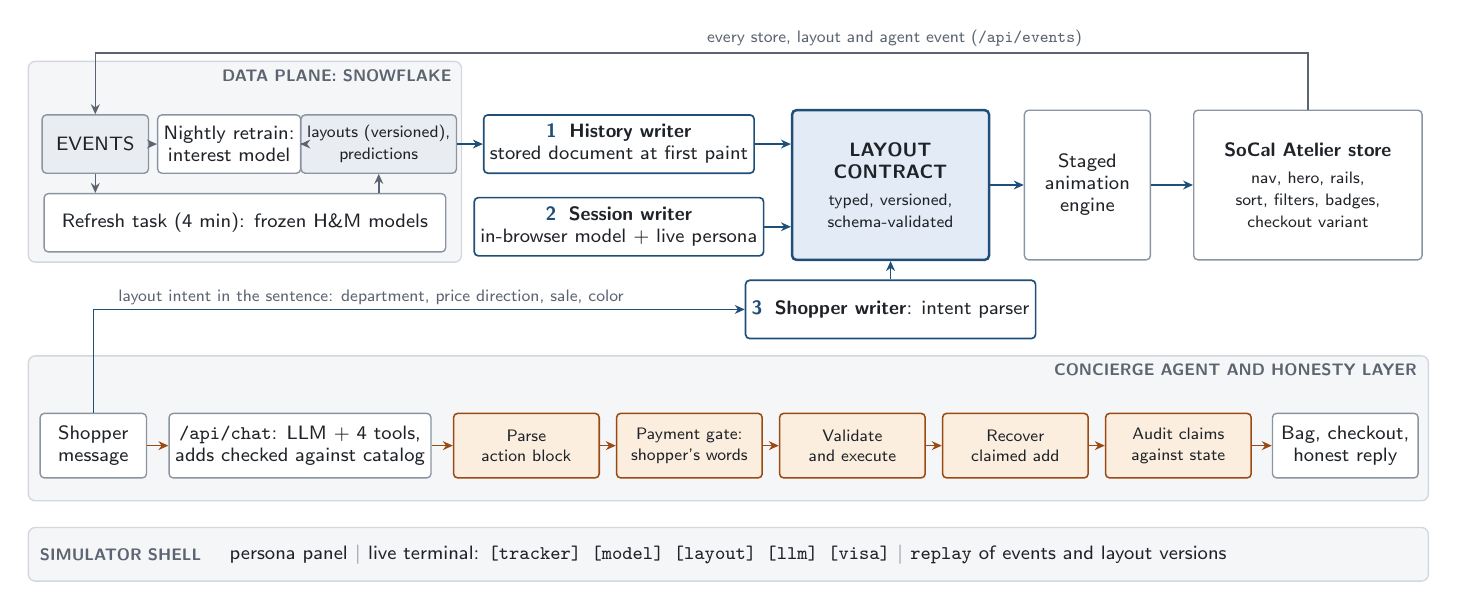
\begin{tikzpicture}[
    x=1cm, y=1cm, font=\sffamily\fs, text=ink,
    box/.style={draw=line, fill=white, rounded corners=1.5pt, line width=.5pt,
                align=center, inner sep=2.2pt, minimum height=.74cm},
    data/.style={box, fill=store},
    writer/.style={box, draw=accent, line width=.6pt},
    chip/.style={box, draw=warm, fill=warmfill, line width=.55pt, minimum width=1.85cm, minimum height=.82cm, font=\sffamily\fontsize{6.4}{7.5}\selectfont},
    lanebox/.style={draw=lanerule, fill=lane, rounded corners=2.5pt, line width=.5pt},
    title/.style={font=\sffamily\ftitle, text=muted, inner sep=0pt},
    flow/.style={-{Stealth[length=3.6pt,width=3.2pt]}, draw=muted, line width=.55pt},
    lflow/.style={flow, draw=accent},
    aflow/.style={flow, draw=warm},
    note/.style={font=\sffamily\fsmall, text=muted, inner sep=1pt},
  ]

  % ---------------------------------------------------------------- lanes
  \path[lanebox] (0,4.05) rectangle (5.5,6.6);
  \node[title, anchor=north east] at (5.38,6.5) {DATA PLANE: SNOWFLAKE};
  \path[lanebox] (0,1.02) rectangle (17.78,2.86);
  \node[title, anchor=north east] at (17.64,2.76) {CONCIERGE AGENT AND HONESTY LAYER};
  \path[lanebox] (0,0) rectangle (17.78,.68);

  % ---------------------------------------------------------------- data plane
  \node[data, minimum width=1.35cm] (ev) at (.85,5.55) {EVENTS};
  \node[box,  minimum width=1.7cm] (nr) at (2.55,5.55) {Nightly retrain:\\interest model};
  \node[data, minimum width=1.8cm] (ul) at (4.45,5.55) {{\fsmall layouts (versioned),}\\{\fsmall predictions}};
  \node[box,  minimum width=5.1cm] (rt) at (2.75,4.55)
    {Refresh task (4 min): frozen H\&M models};
  \draw[flow] (ev) -- (nr);
  \draw[flow] (nr) -- (ul);
  \draw[flow] (ev.south) -- (ev.south |- rt.north);
  \draw[flow] (ul.south |- rt.north) -- (ul.south);

  % ---------------------------------------------------------------- writers and contract
  \node[writer, minimum width=3.3cm] (w1) at (7.5,5.55)
    {\wnum{1}\; \textbf{History writer}\\stored document at first paint};
  \node[writer, minimum width=3.3cm] (w2) at (7.5,4.5)
    {\wnum{2}\; \textbf{Session writer}\\in-browser model + live persona};
  \node[box, draw=accent, fill=accentfill, line width=.9pt, minimum width=2.5cm, minimum height=1.9cm]
    (c) at (10.95,5.03) {\textbf{LAYOUT}\\\textbf{CONTRACT}\\[2pt]{\fsmall typed, versioned,}\\{\fsmall schema-validated}};
  \node[box, minimum width=1.6cm, minimum height=1.9cm] (an) at (13.45,5.03) {Staged\\animation\\engine};
  \node[box, minimum width=2.9cm, minimum height=1.9cm] (st) at (16.25,5.03)
    {\textbf{SoCal Atelier store}\\[2pt]{\fsmall nav, hero, rails,}\\{\fsmall sort, filters, badges,}\\{\fsmall checkout variant}};

  \draw[lflow] (ul) -- (w1) node[note, midway, above=1pt] {};
  \draw[lflow] (w1.east) -- (w1.east -| c.west);
  \draw[lflow] (w2.east) -- (w2.east -| c.west);
  \draw[lflow] (c) -- (an);
  \draw[lflow] (an) -- (st);

  % store events flow back to the warehouse along the top
  \draw[flow] (st.north) -- ++(0,.72) -| (ev.north);
  \node[note, anchor=south] at (11.0,6.74) {every store, layout and agent event (\texttt{/api/events})};

  % ---------------------------------------------------------------- agent lane
  \node[box, minimum width=1.35cm, minimum height=.82cm] (sm) at (.825,1.72) {Shopper\\message};
  \node[box, minimum width=3.3cm, minimum height=.82cm] (ch) at (3.45,1.72)
    {\texttt{/api/chat}: LLM + 4 tools,\\adds checked against catalog};
  \node[chip] (p1) at (6.325,1.72) {Parse\\action block};
  \node[chip] (p2) at (8.395,1.72) {Payment gate:\\shopper's words};
  \node[chip] (p3) at (10.465,1.72) {Validate\\and execute};
  \node[chip] (p4) at (12.535,1.72) {Recover\\claimed add};
  \node[chip] (p5) at (14.605,1.72) {Audit claims\\against state};
  \node[box, minimum width=1.85cm, minimum height=.82cm] (out) at (16.725,1.72)
    {Bag, checkout,\\honest reply};
  \draw[aflow] (sm) -- (ch);
  \draw[aflow] (ch) -- (p1);
  \draw[aflow] (p1) -- (p2);
  \draw[aflow] (p2) -- (p3);
  \draw[aflow] (p3) -- (p4);
  \draw[aflow] (p4) -- (p5);
  \draw[aflow] (p5) -- (out);

  % ---------------------------------------------------------------- shopper writer
  \node[writer, minimum width=3.3cm] (w3) at (10.95,3.45)
    {\wnum{3}\; \textbf{Shopper writer}: intent parser};
  \draw[lflow] (sm.north) |- (w3.west);
  \draw[lflow] (w3) -- (c);
  \node[note, anchor=south west] at (1.1,3.47) {layout intent in the sentence: department, price direction, sale, color};

  % ---------------------------------------------------------------- shell
  \node[title, anchor=west] at (.14,.34) {SIMULATOR SHELL};
  \node[anchor=west, inner sep=0pt] at (2.55,.34)
    {persona panel \textcolor{line}{\textbar} live terminal:
     \texttt{[tracker] [model] [layout] [llm] [visa]} \textcolor{line}{\textbar}
     \texttt{replay} of events and layout versions};
\end{tikzpicture}
\end{document}
